\documentclass[12pt,a4paper]{article}
\usepackage[margin=2cm]{geometry}
\usepackage{amsmath,amsthm,amssymb}
\usepackage{CJK}
\usepackage{verbatim}
\usepackage{graphicx}

\begin{document}
	\begin{CJK}{UTF8}{bsmi}
		\begin{enumerate}
			\item 增厚:
			\begin{figure}[htbp]
				\centering
				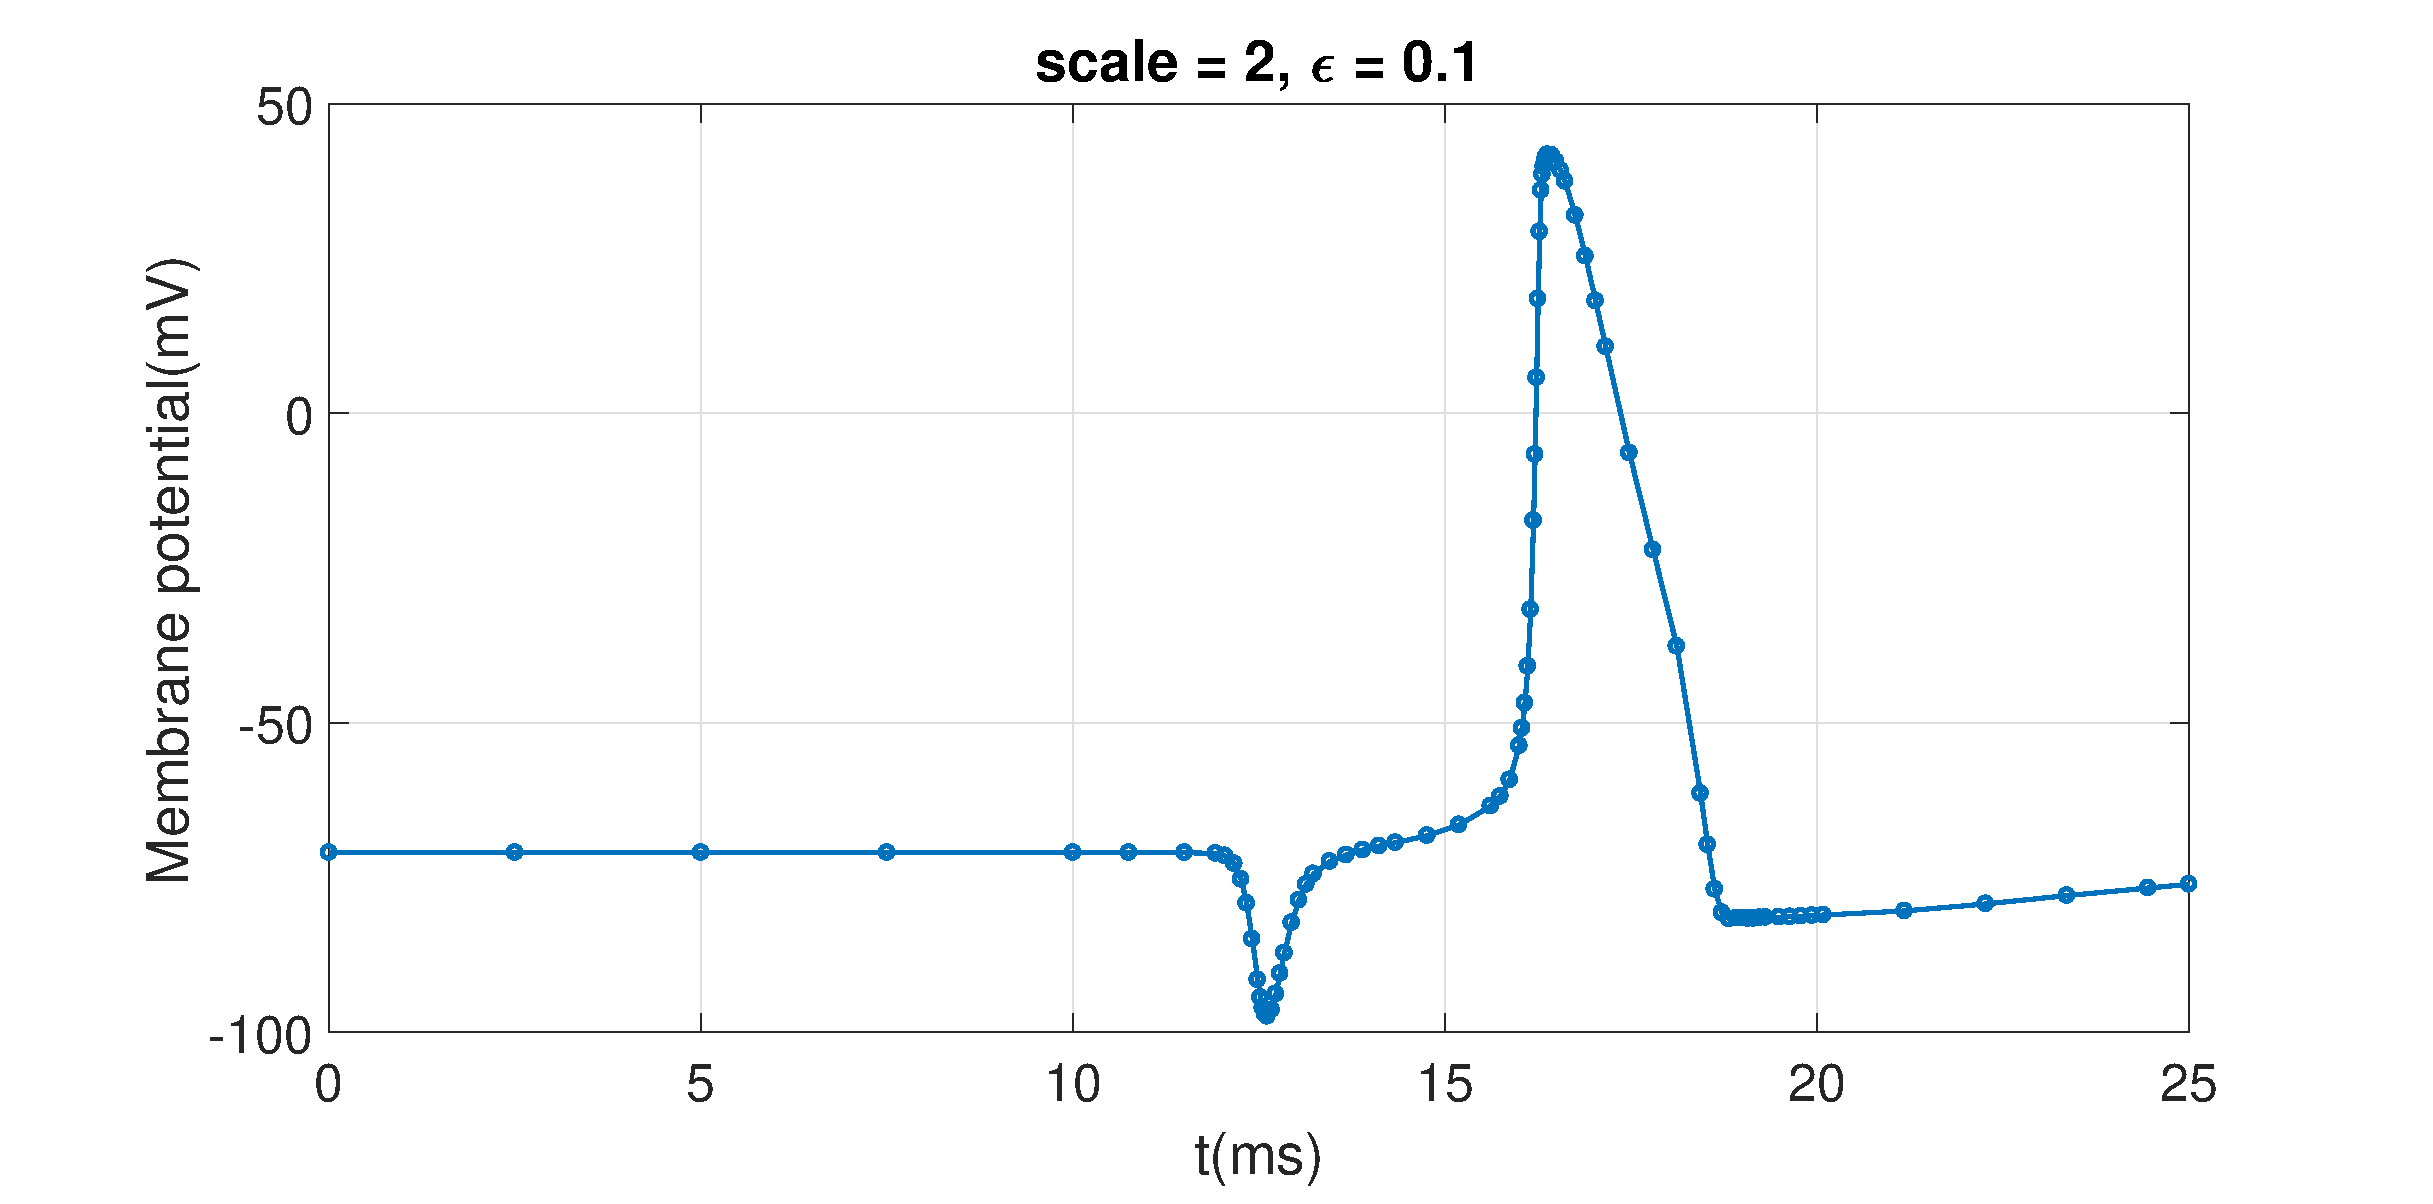
\includegraphics[width = 500pt]{AP1.eps}
			\end{figure}
			\newpage
			電流比較:\\
			\begin{figure}[htbp]
				\centering
				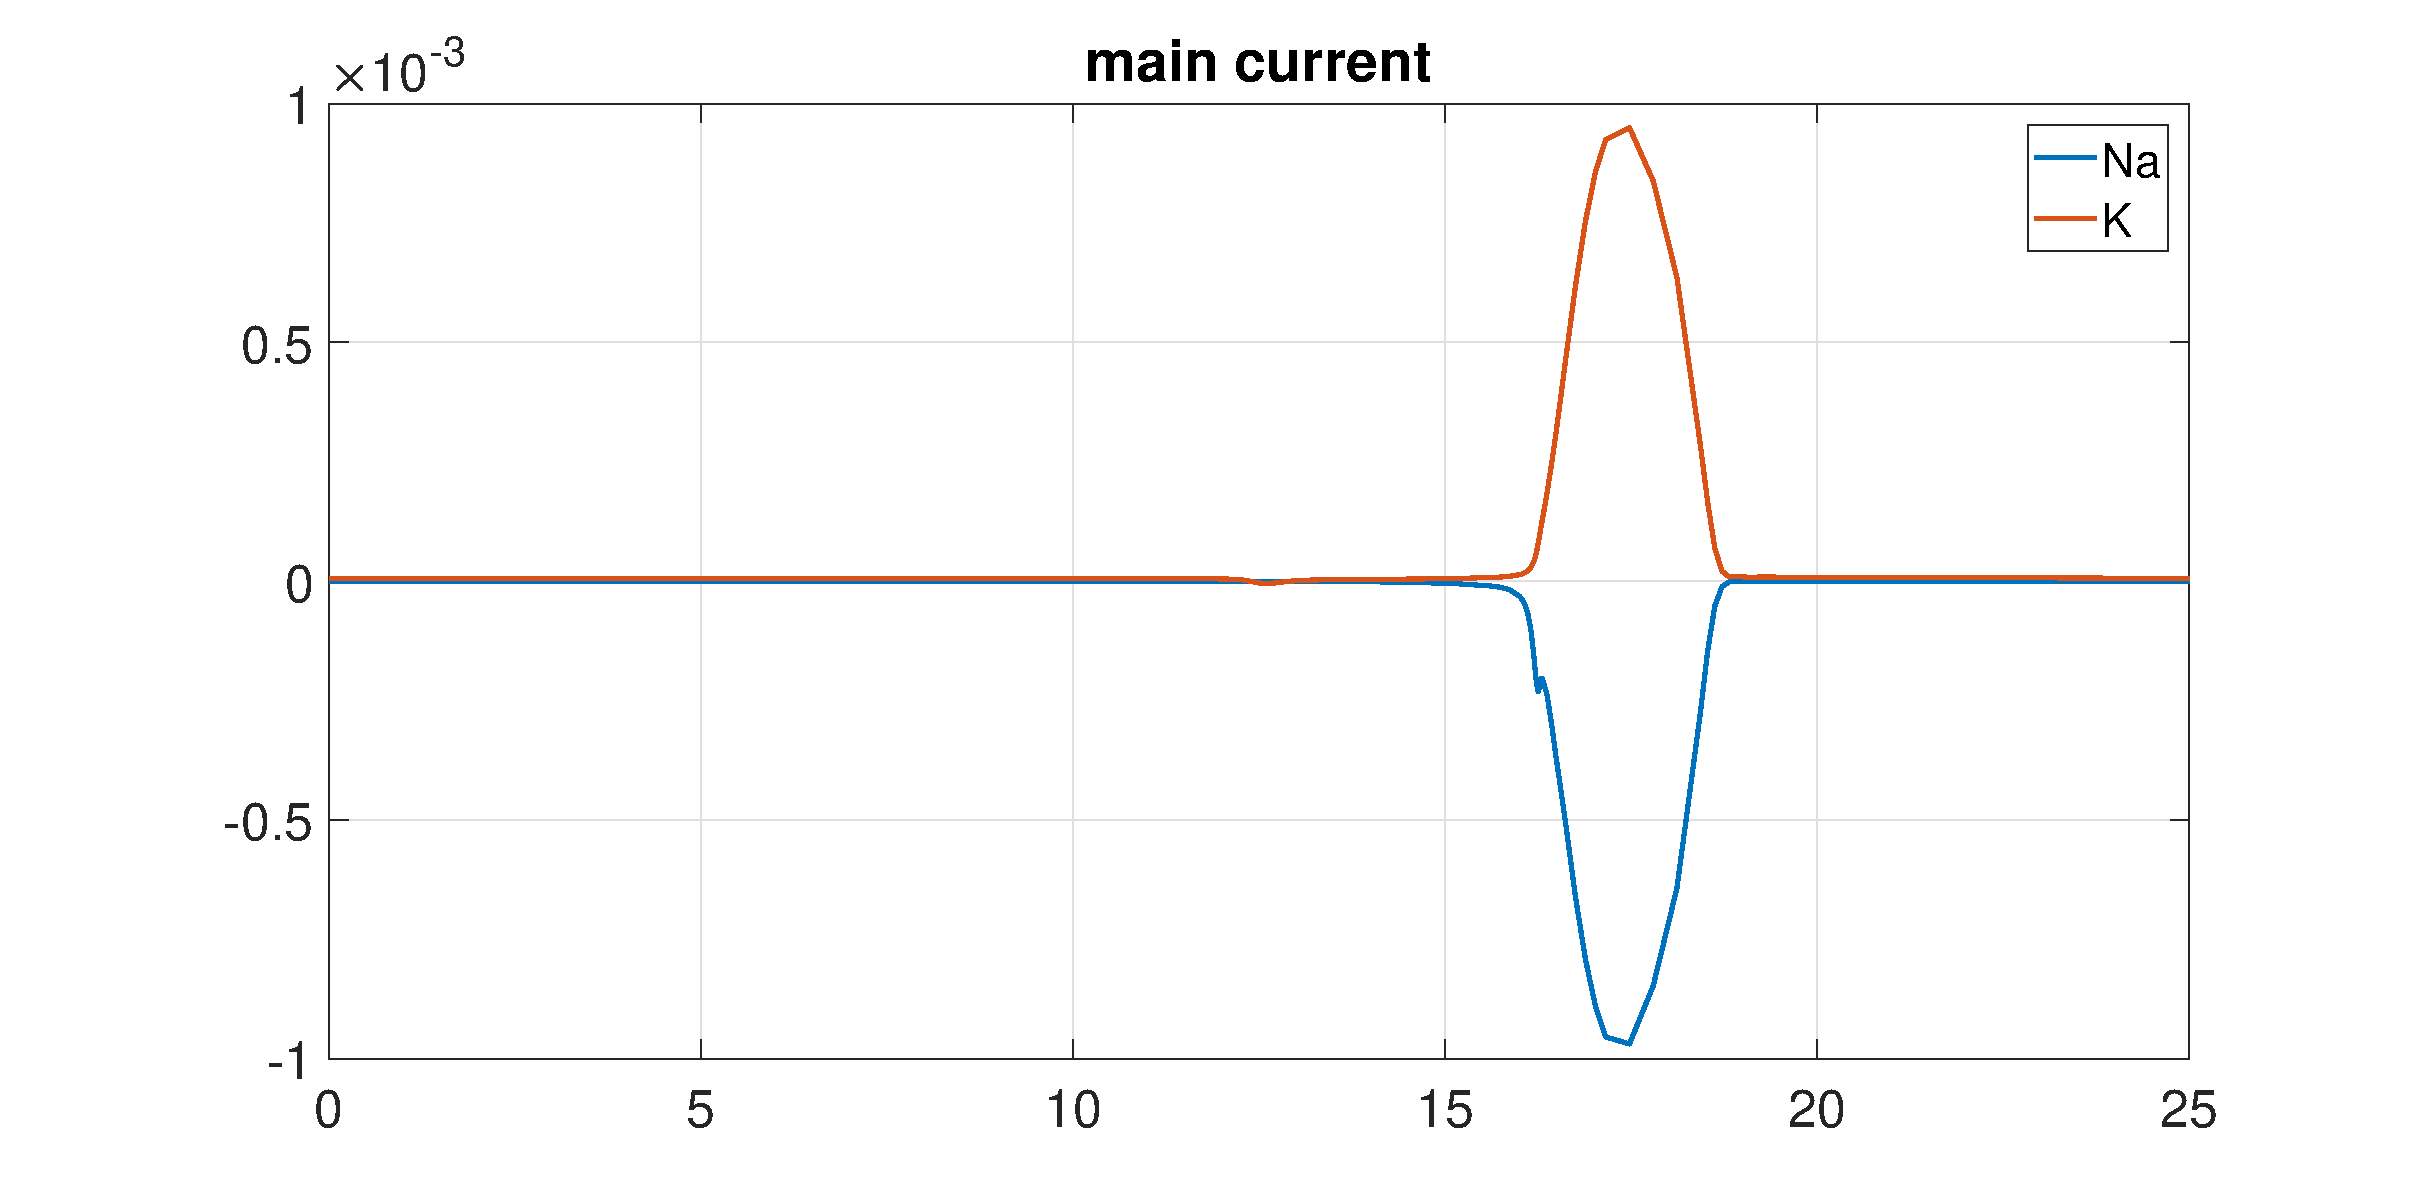
\includegraphics[width = 500pt]{main1.eps}
			\end{figure}
			\begin{figure}[htbp]
				\centering
				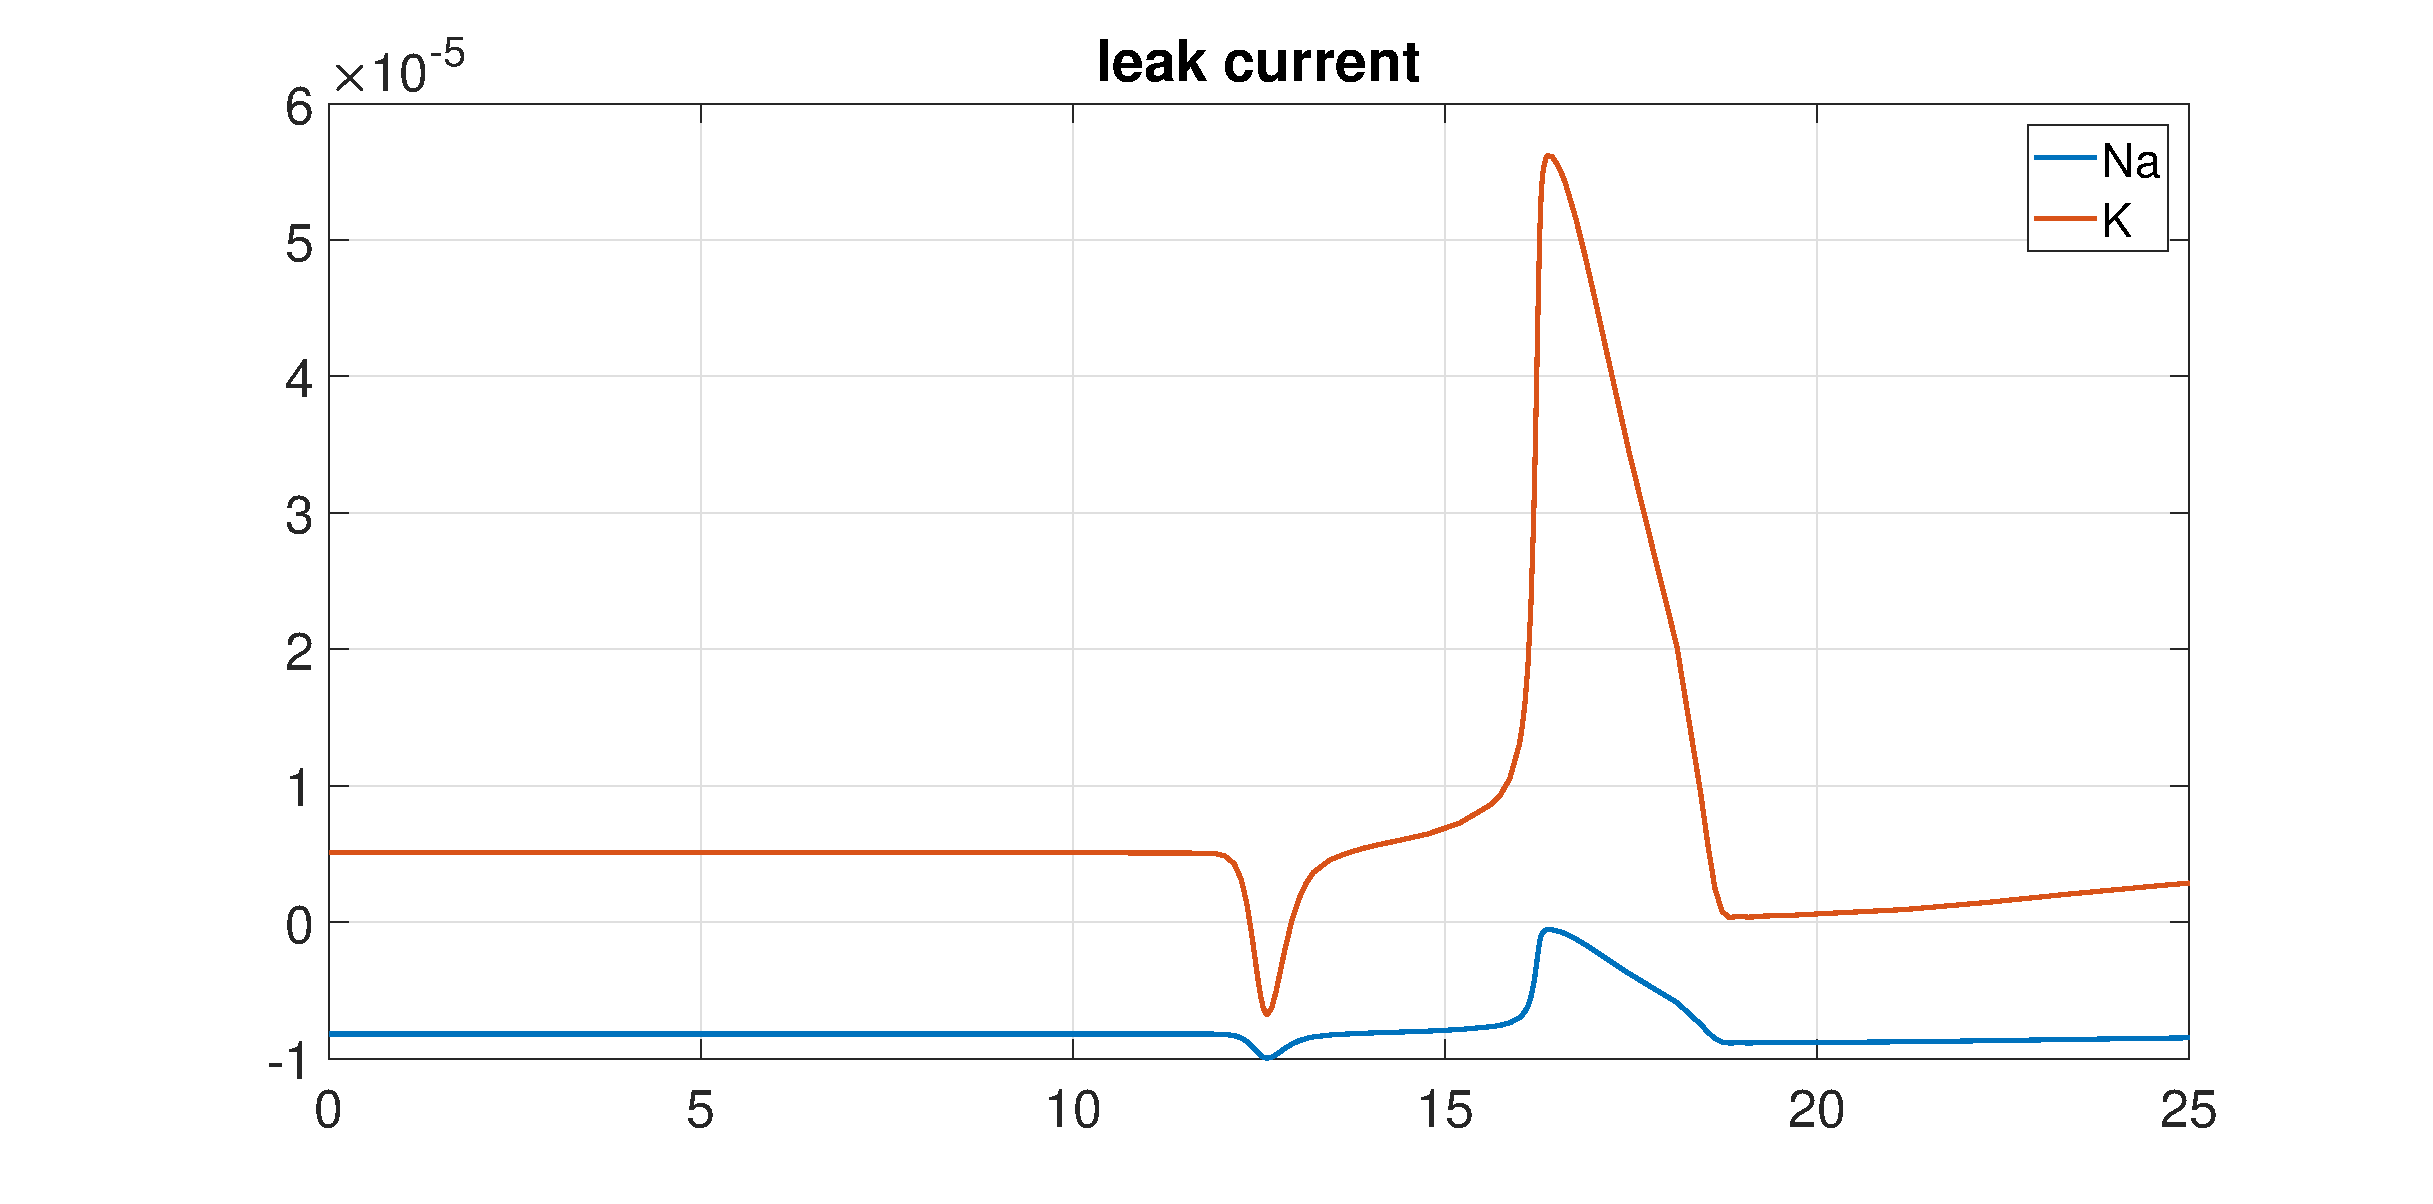
\includegraphics[width = 500pt]{leak1.eps}
			\end{figure}
			\newpage
			gating variables之比較:\\
			\begin{figure}[htbp]
				\centering
				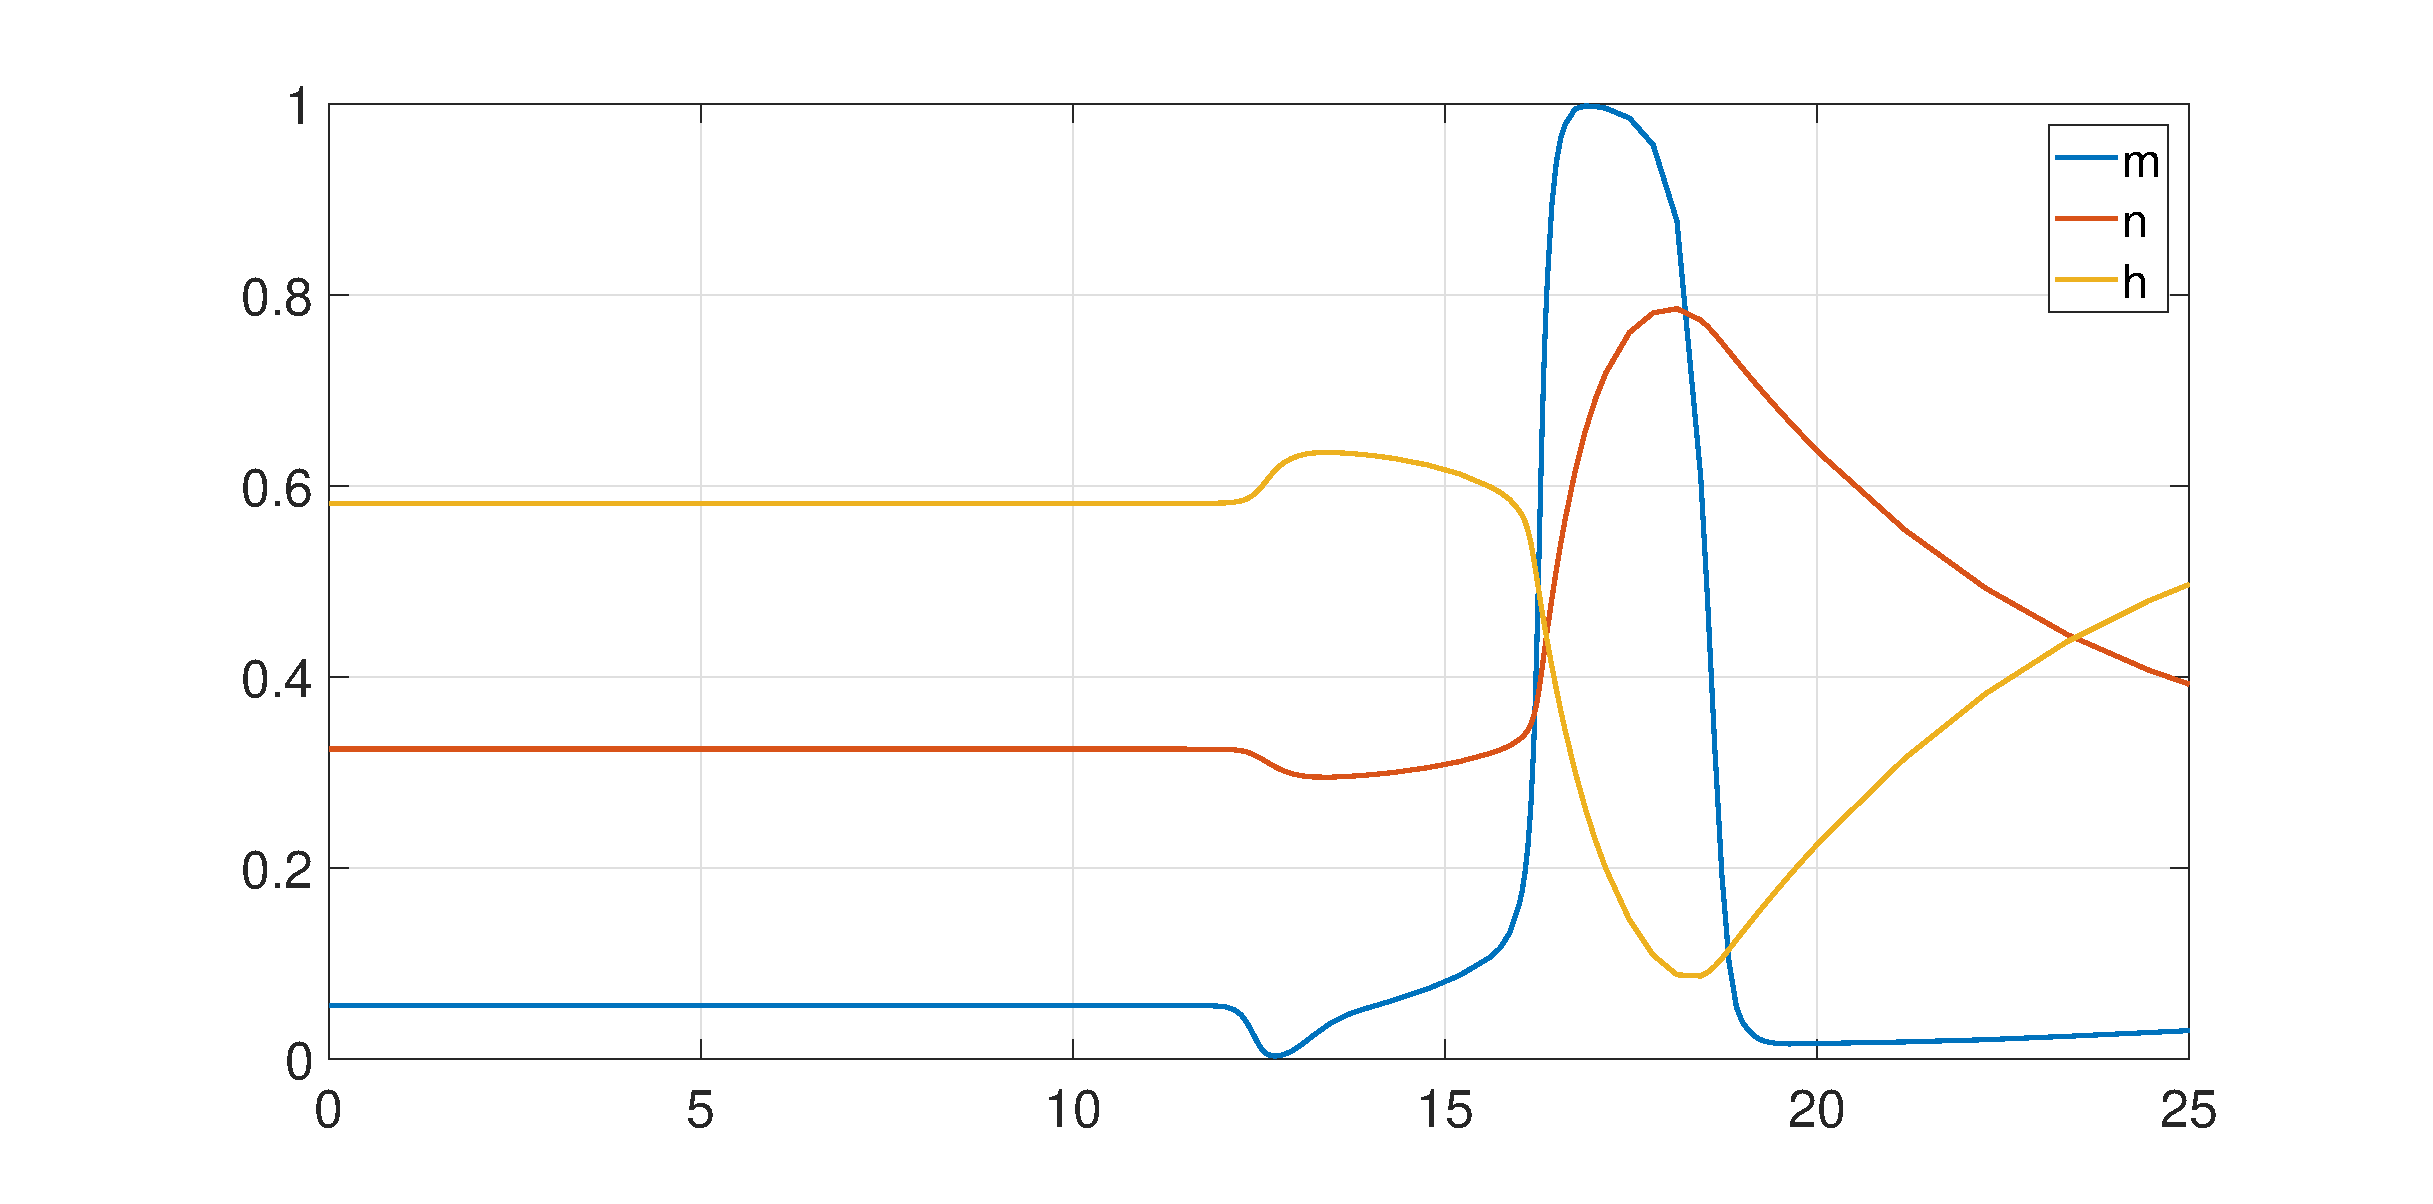
\includegraphics[width = 500pt]{mnh1.eps}
			\end{figure}
			\begin{figure}[htbp]
				\centering
				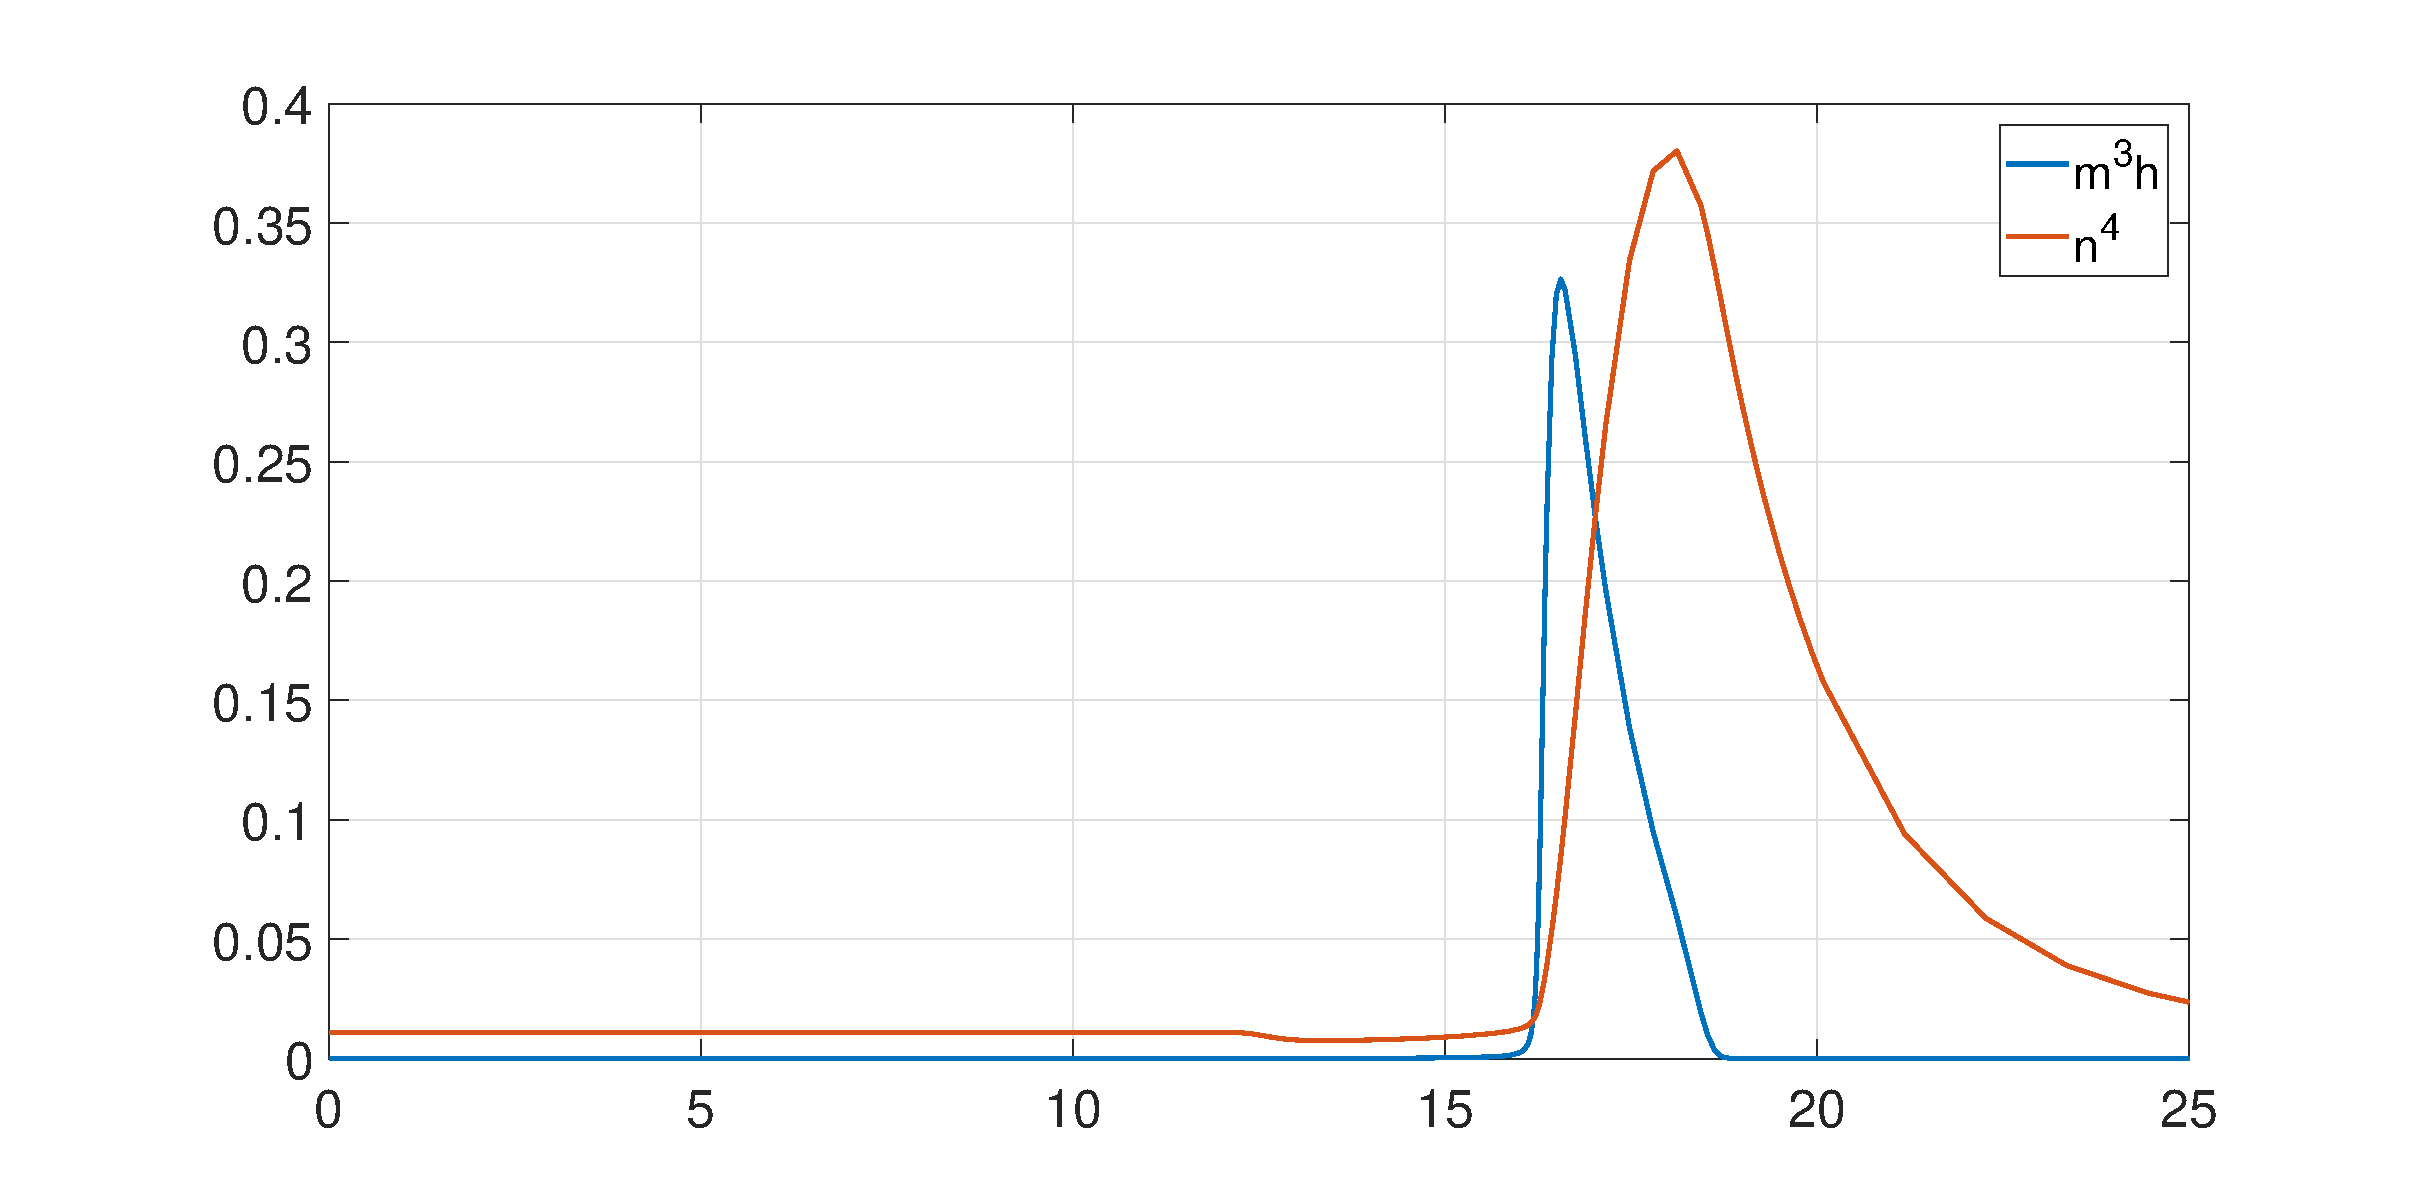
\includegraphics[width = 500pt]{gate1.eps}
			\end{figure}
			\newpage
			\item 變薄:
			\begin{figure}[htbp]
				\centering
				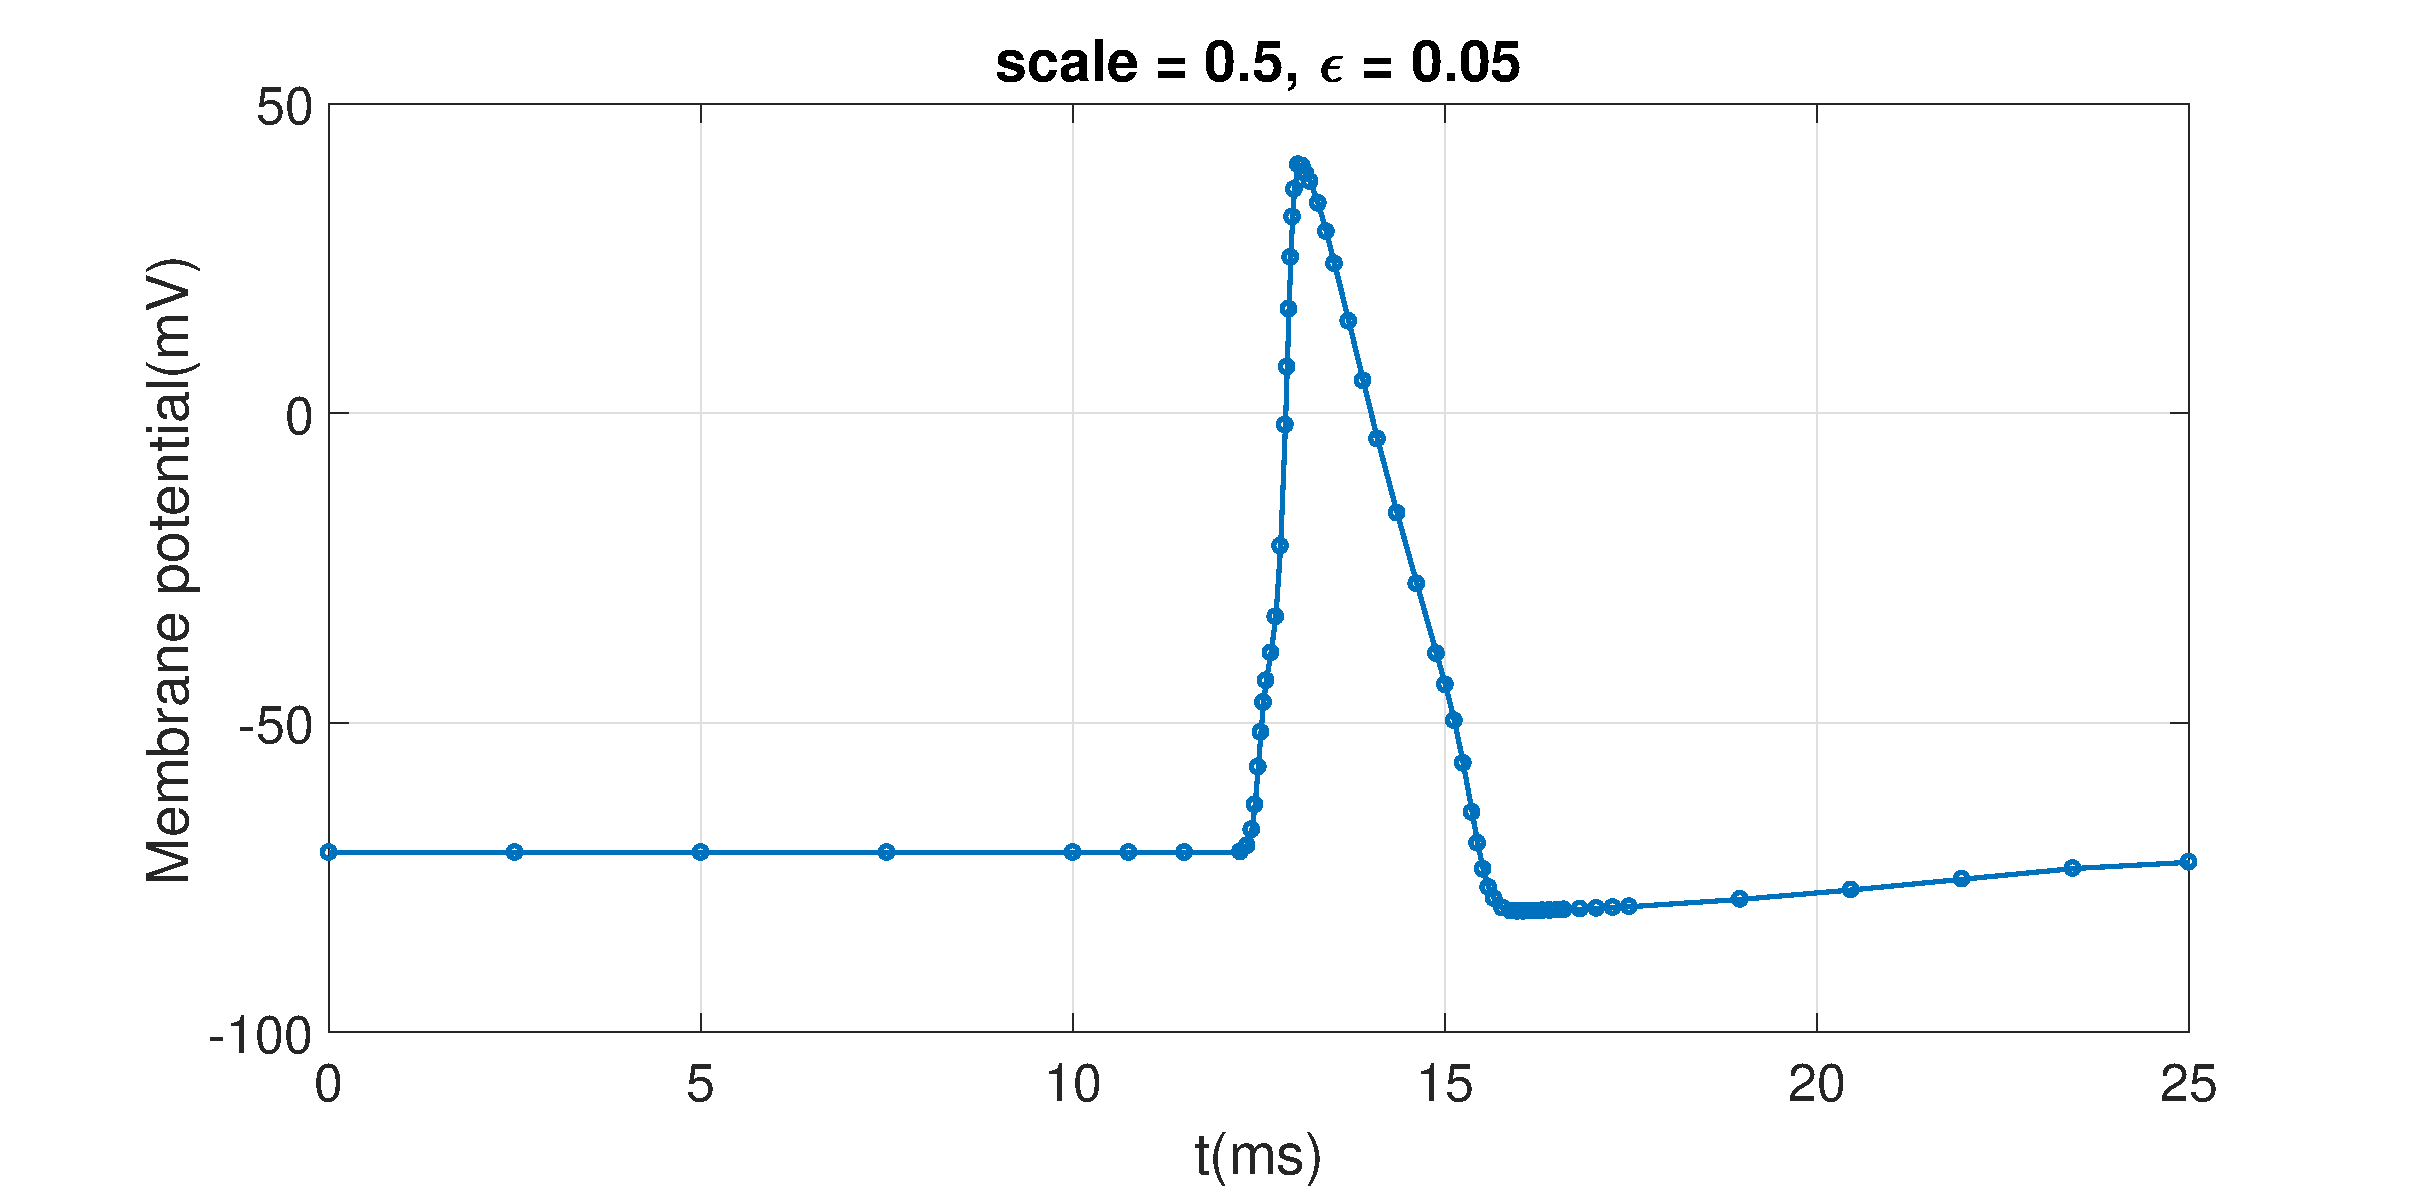
\includegraphics[width = 500pt]{AP2.eps}
			\end{figure}
			\newpage
			電流比較:\\
			\begin{figure}[htbp]
				\centering
				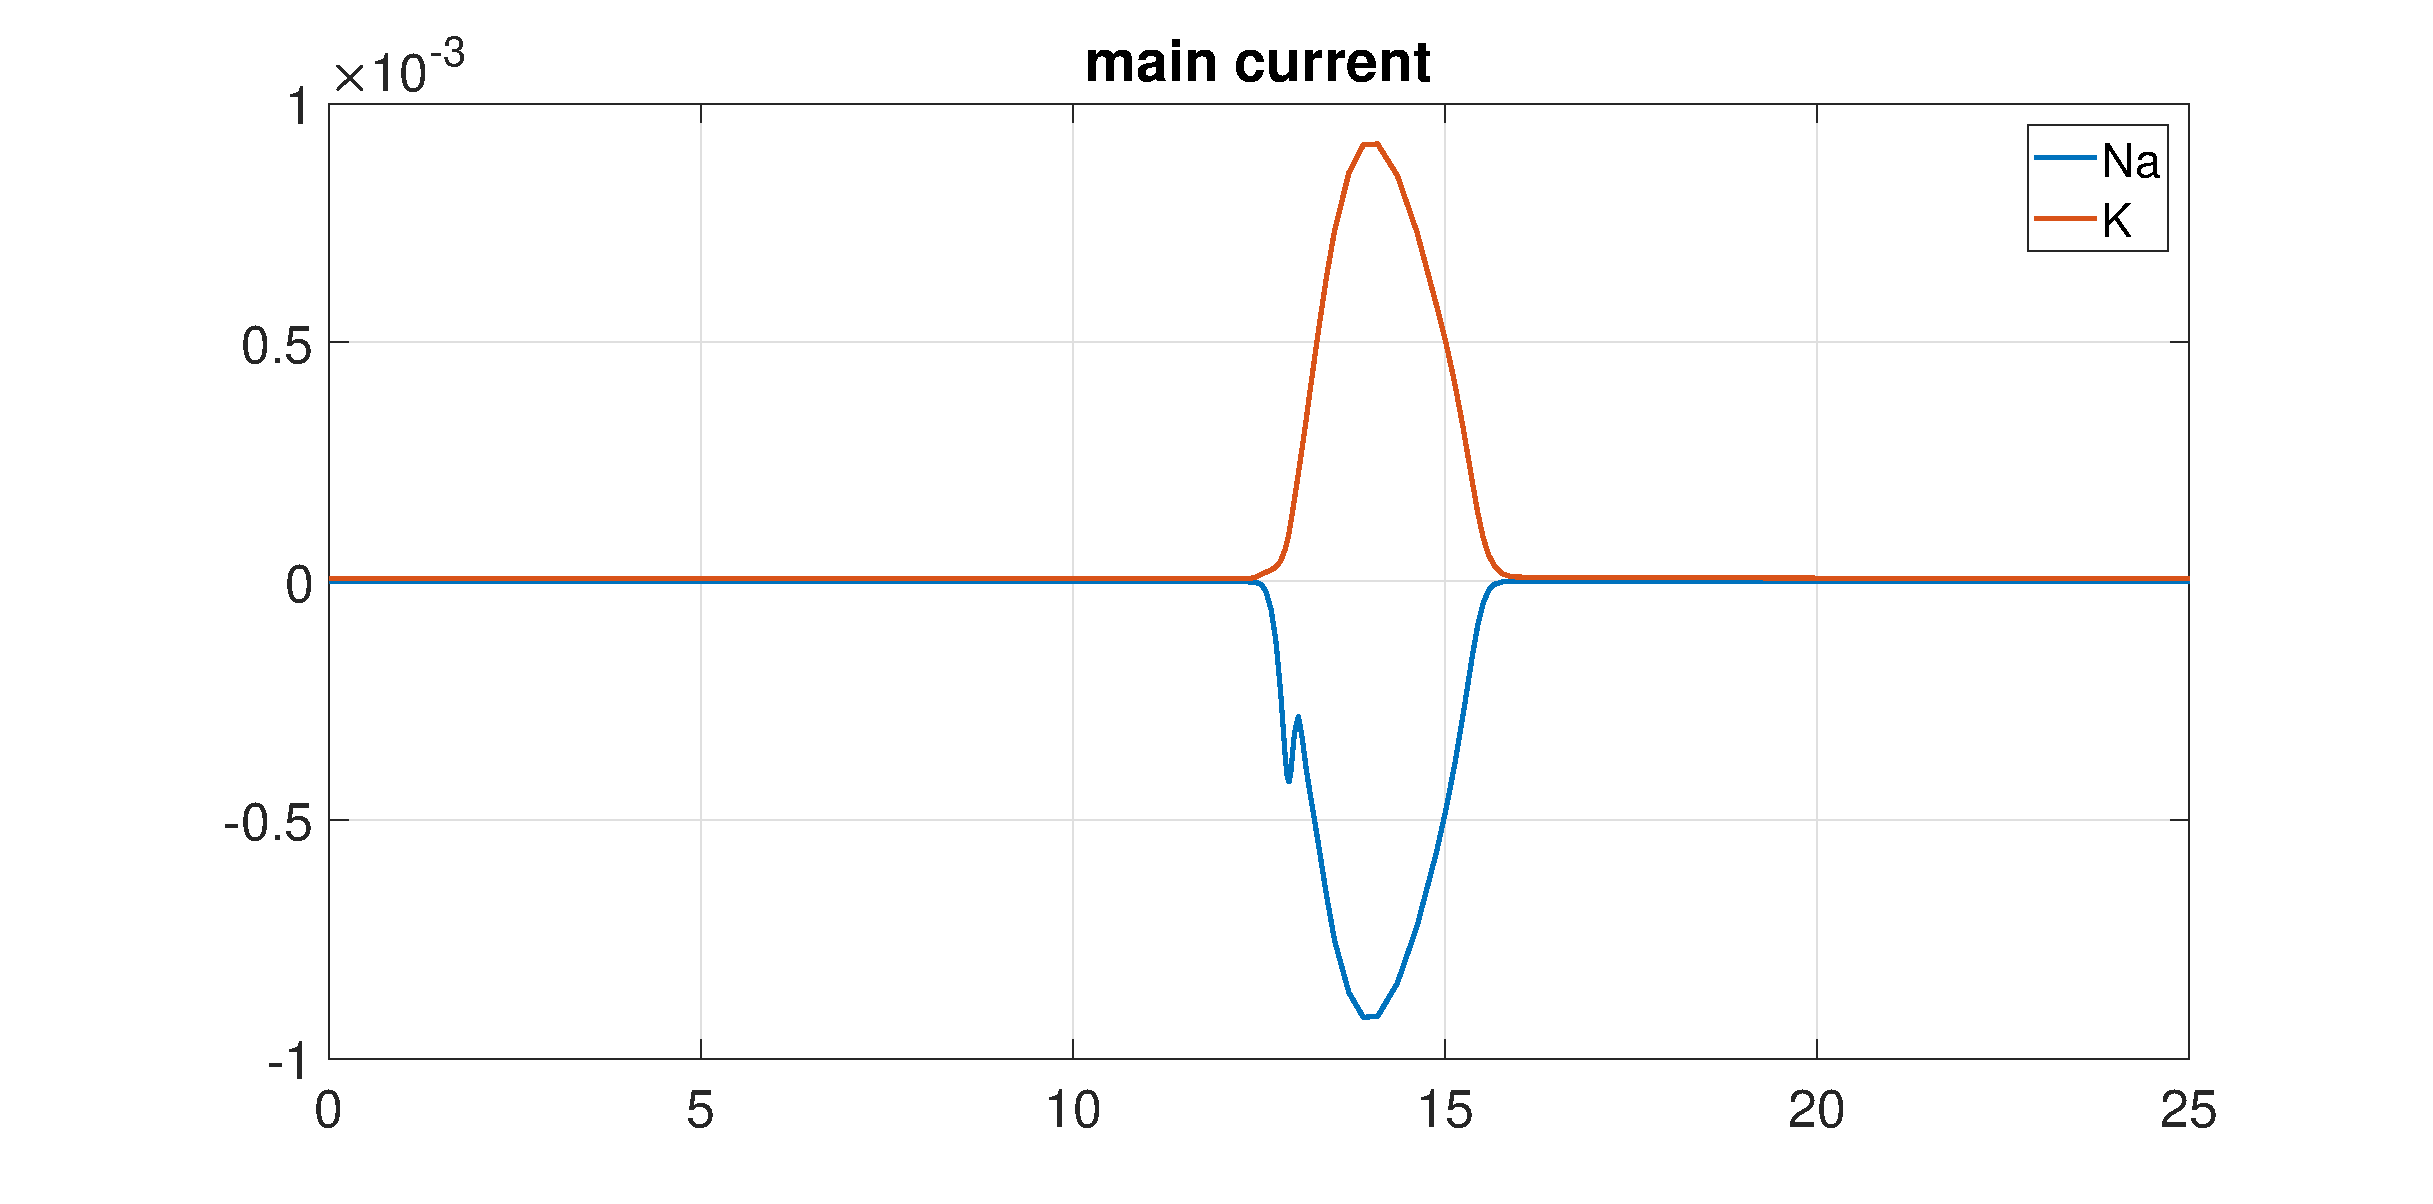
\includegraphics[width = 500pt]{main2.eps}
			\end{figure}
			\begin{figure}[htbp]
				\centering
				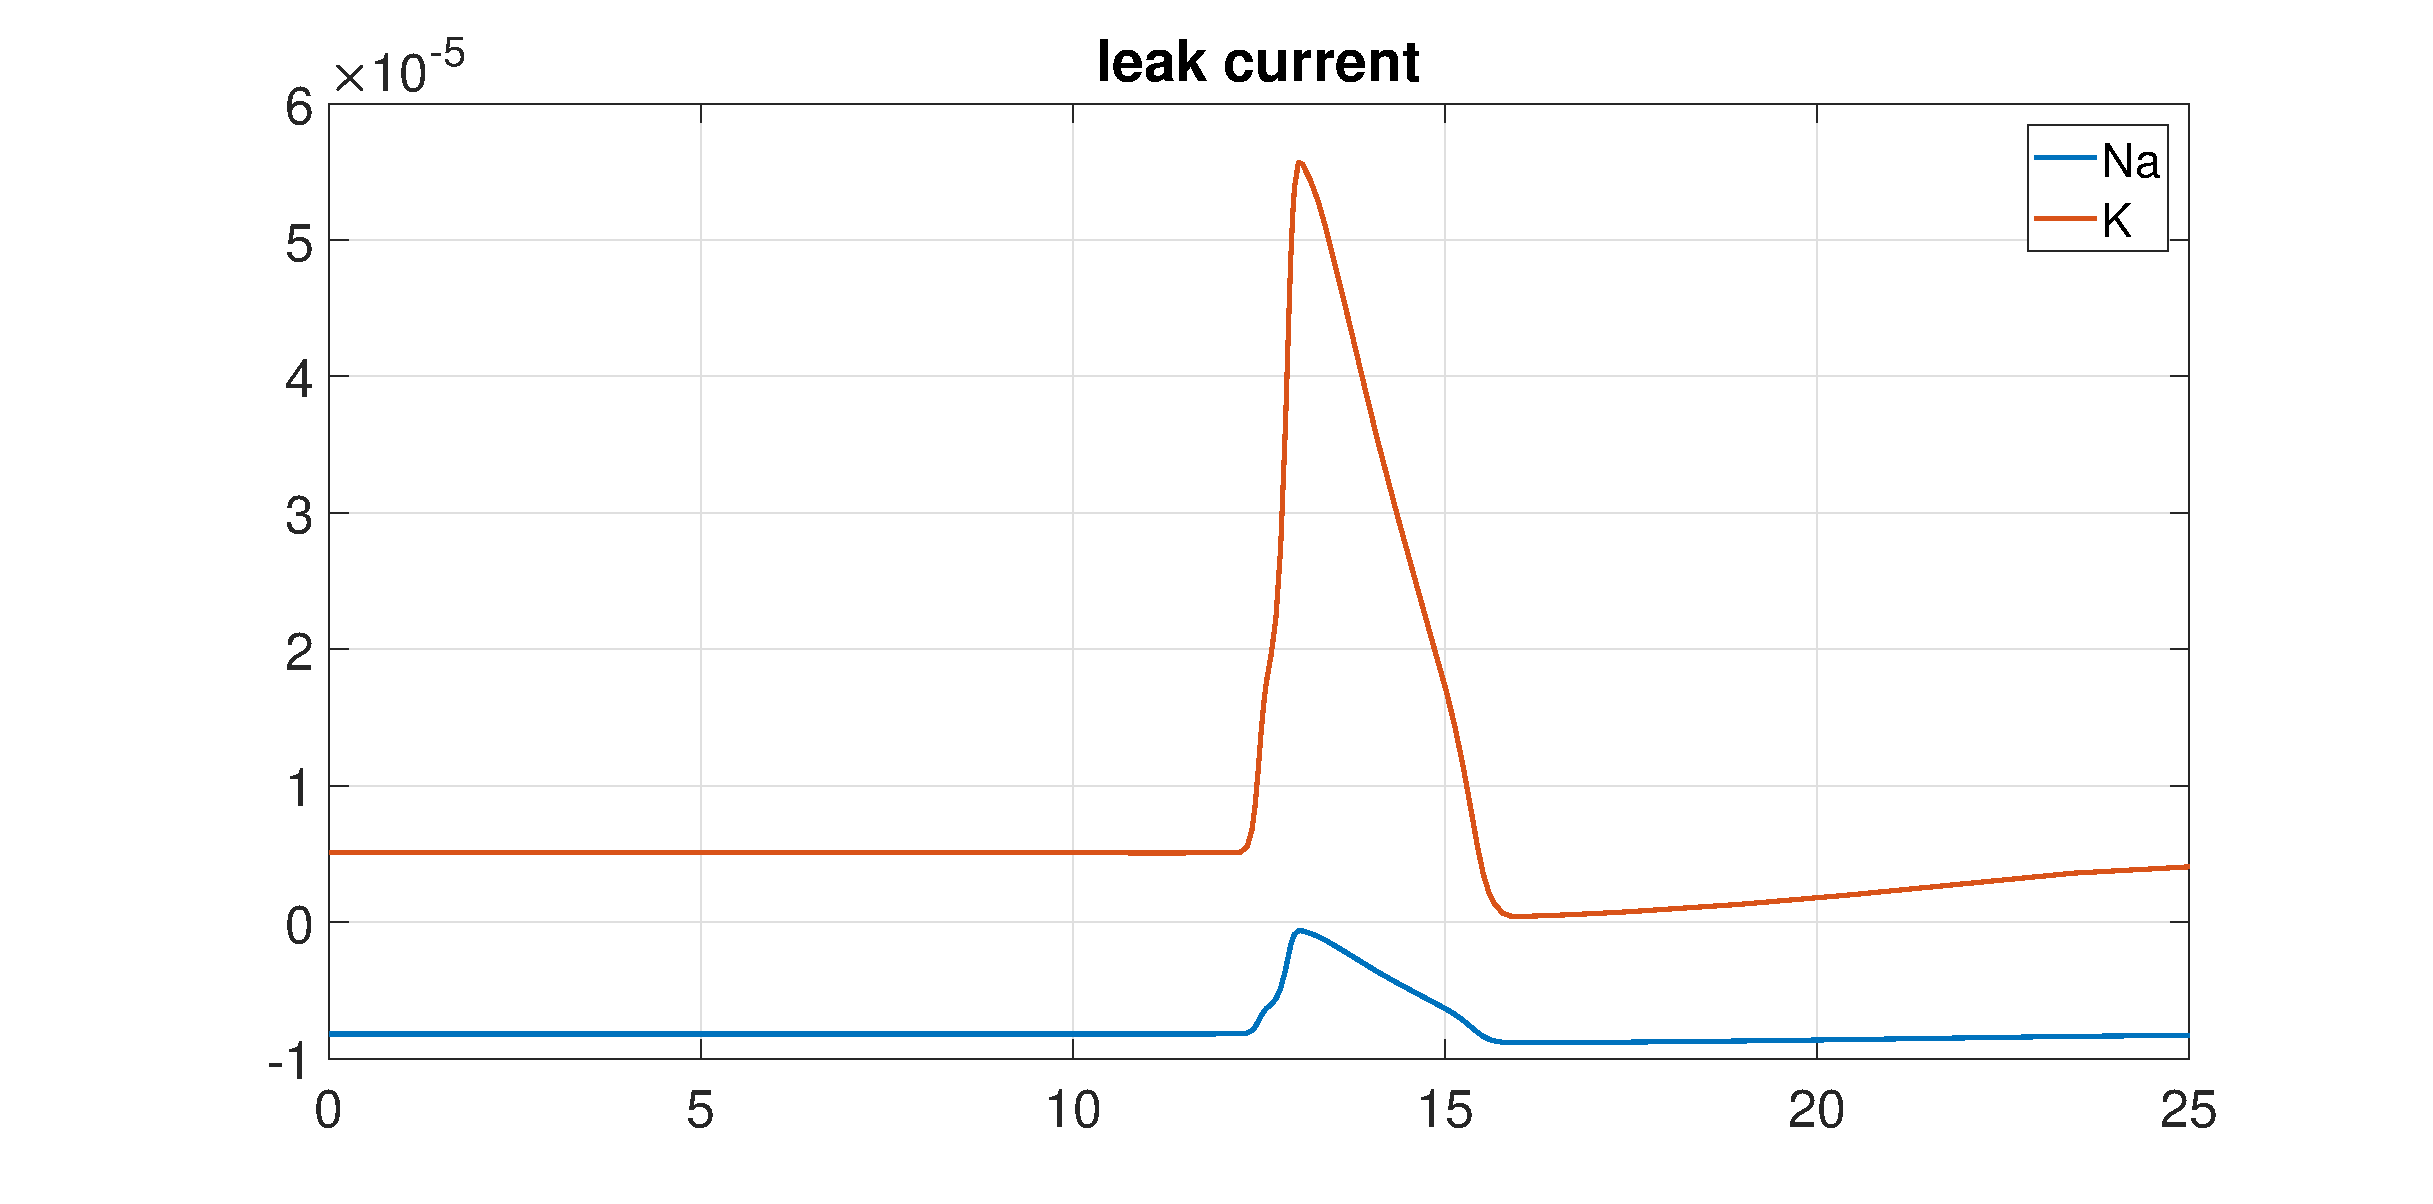
\includegraphics[width = 500pt]{leak2.eps}
			\end{figure}
			\newpage
			gating variables之比較:\\
			\begin{figure}[htbp]
				\centering
				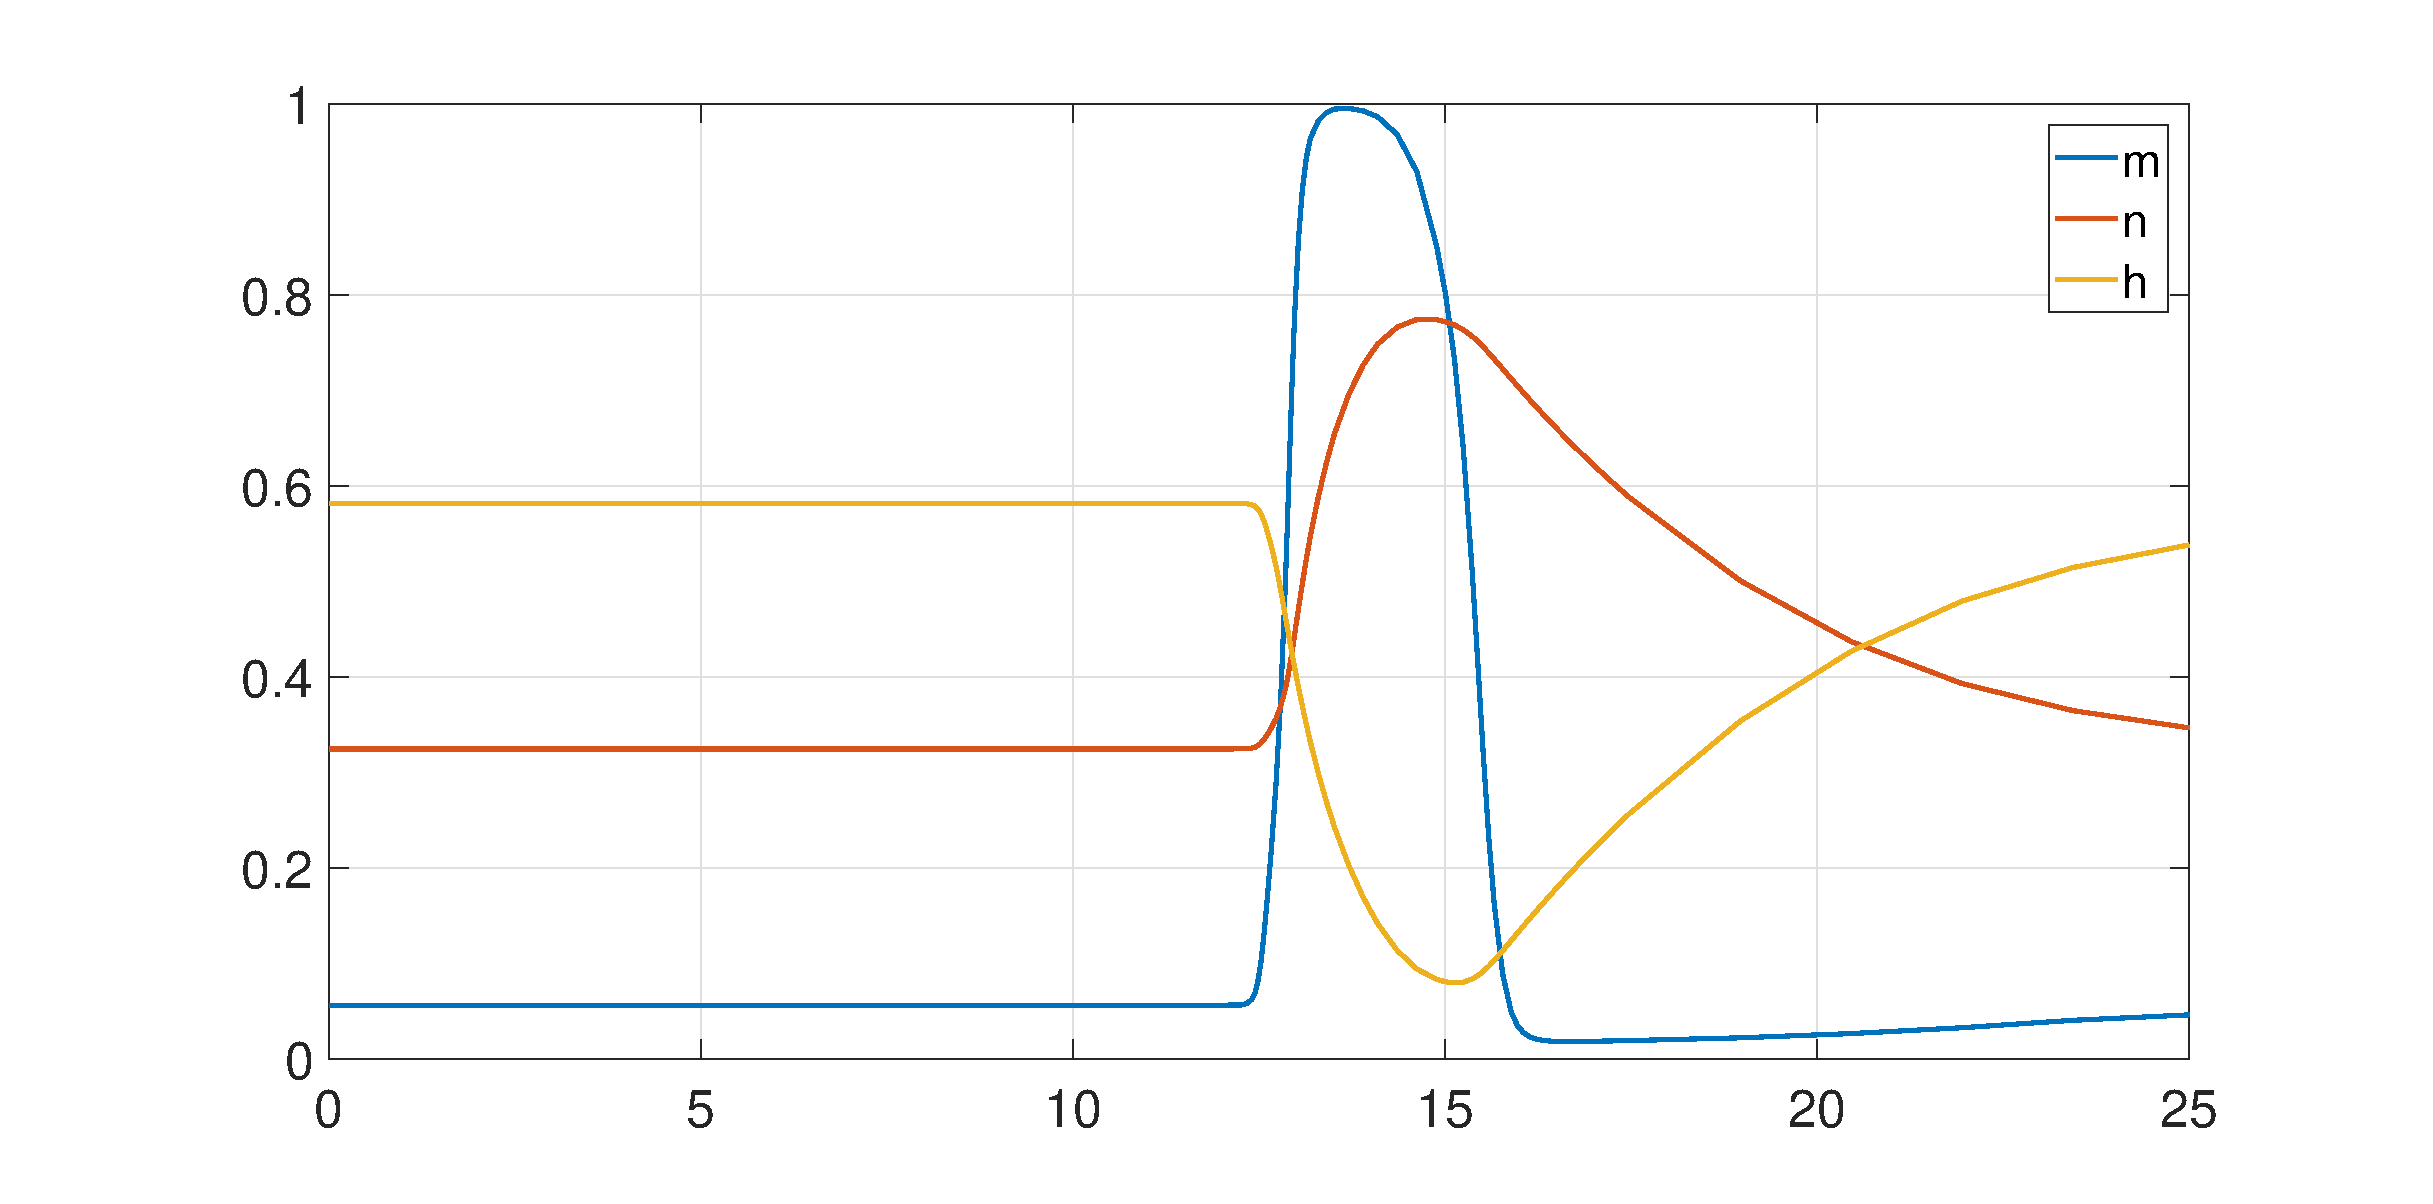
\includegraphics[width = 500pt]{mnh2.eps}
			\end{figure}
			\begin{figure}[htbp]
				\centering
				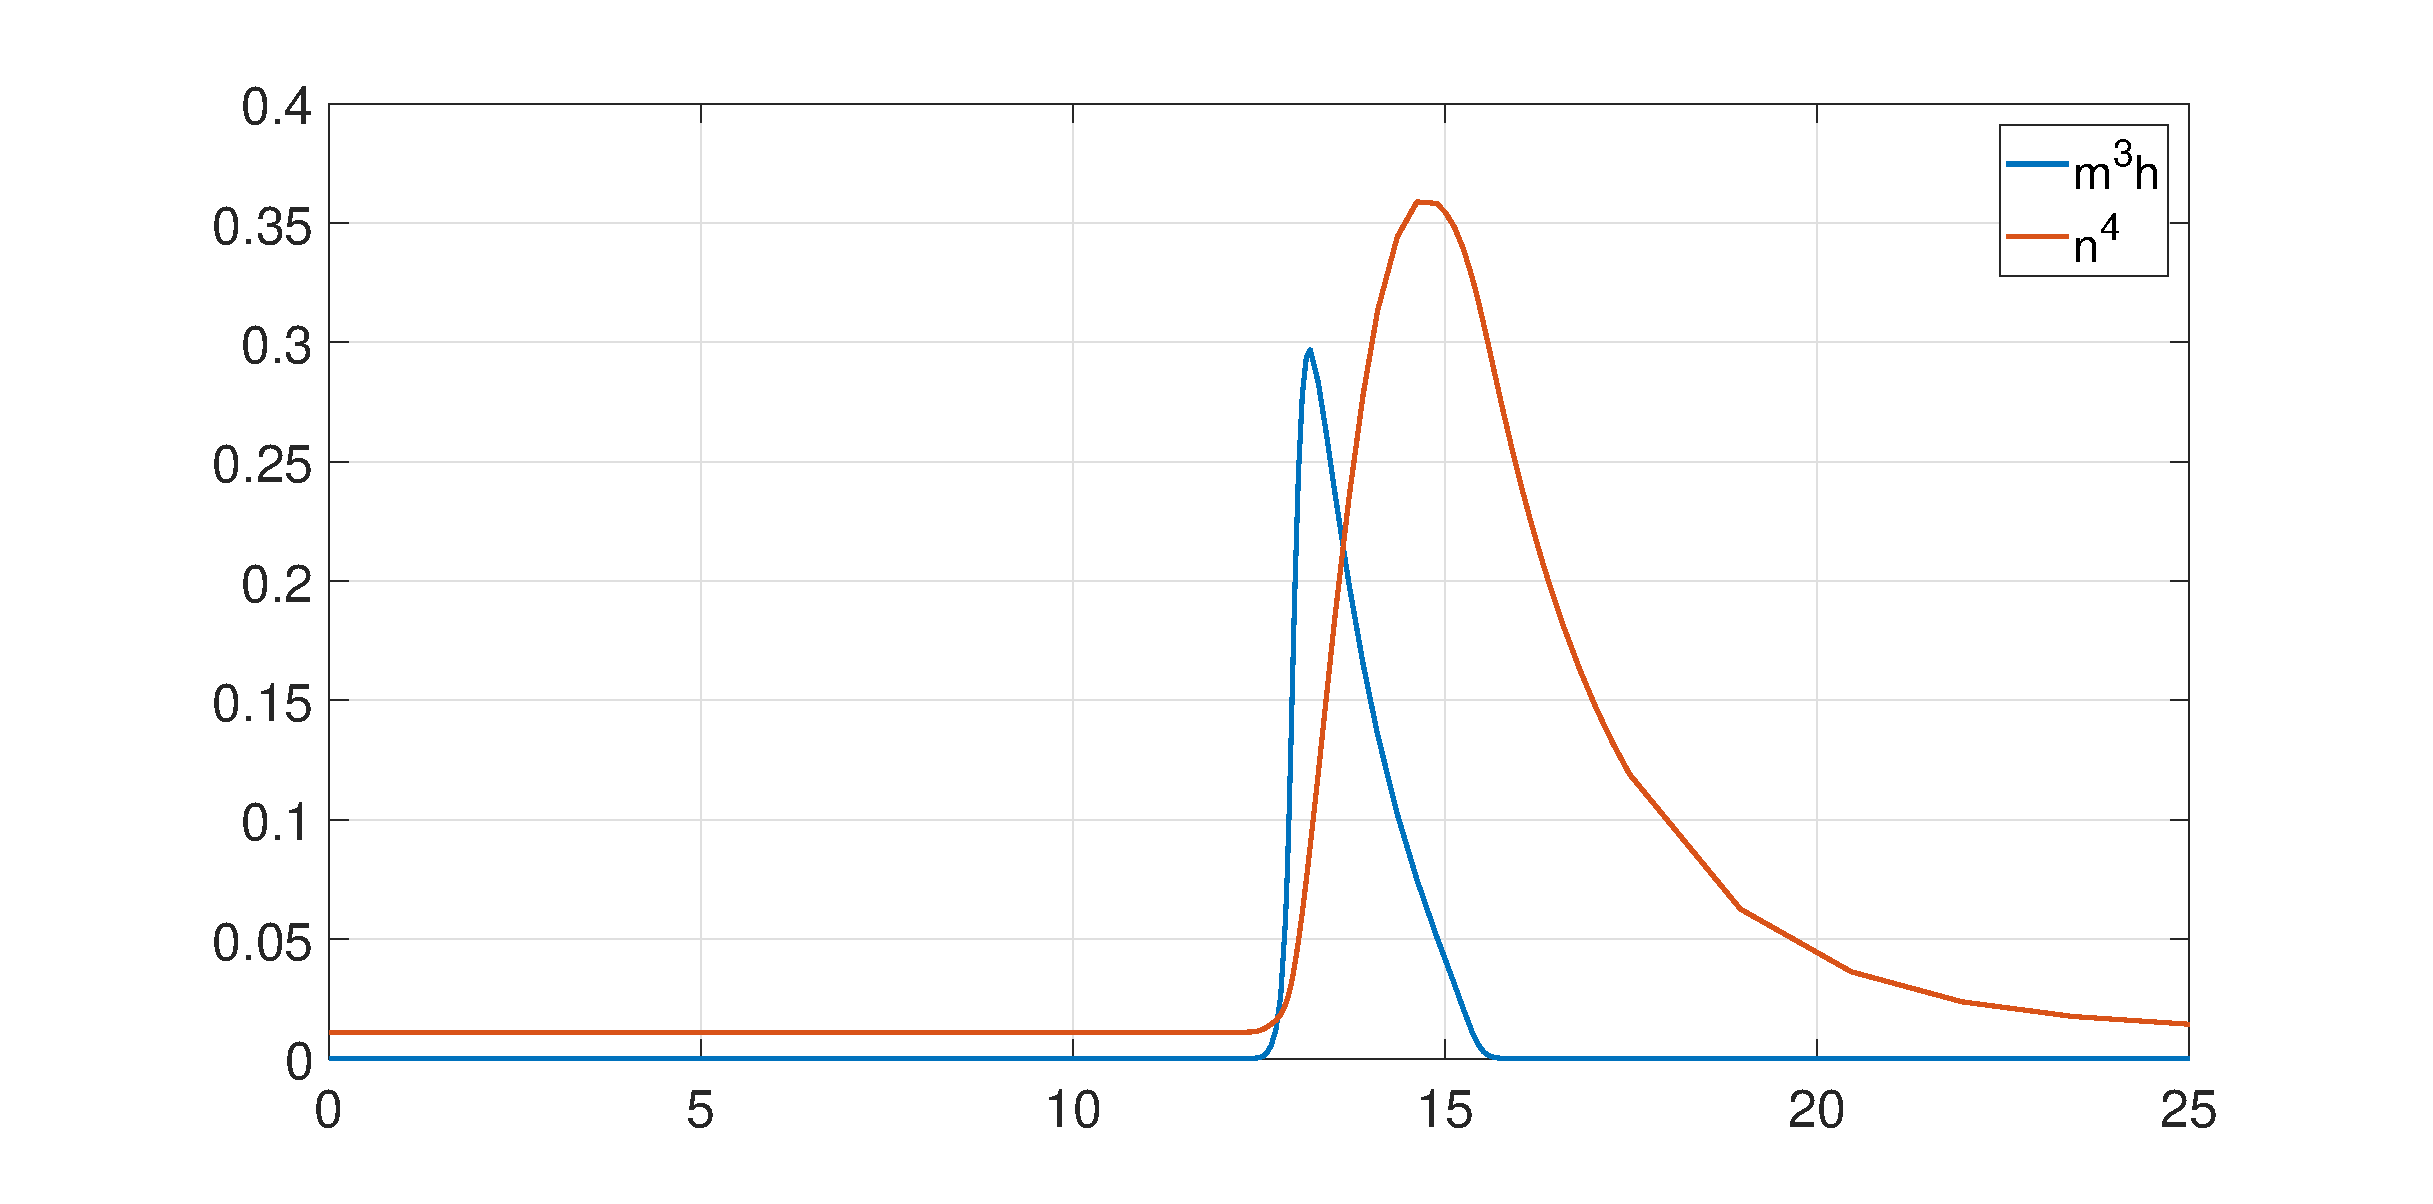
\includegraphics[width = 500pt]{gate2.eps}
			\end{figure}
		\end{enumerate}
	\end{CJK}
\end{document}